\section{Born approximation and form factors}\label{sec:2.2}

A dark-matter particle of \SI{100}{MeV} that meets a free electron scatters with the cross-section $\mu_{\chi e}^2|\tilde V|^2/\pi$ when the mediator is heavy. \Cref{sec:1.4} defined $\sigmae$ through this cross-section. The same golden-rule calculation yields the rate off an electron bound in an atom, where the electron's wavefunction enters through a single overlap, the transition form factor, and the rate off a nucleus, whose nucleons scatter in phase and multiply the cross-section by $A^2$. We derive all three from \cref{eq:2.1-golden,eq:2.1-Vbox}, to first order in the potential: the first Born approximation.

\subsection{The Born cross-section}

Take a dark-matter particle and an electron in a box, interacting through a potential $V(\vect{x}_\chi - \vect{x}_e)$ of their separation. Since the total momentum is conserved, it is simplest to work in the center-of-mass frame, where the dark matter has momentum $\vect{p}$, the electron $-\vect{p}$, and the relative speed is $v = p/\mu_{\chi e}$. The kinetic energy of relative motion is $p^2/2\mu_{\chi e}$. In general the Hamiltonian splits as $P_{\mathrm{tot}}^2/2(m_\chi + m_e) + p_{\mathrm{rel}}^2/2\mu_{\chi e} + V(\vect{r})$, with $\vect{P}_{\mathrm{tot}}$ the total momentum, $\vect{p}_{\mathrm{rel}}$ the relative momentum and $\vect{r}$ the separation. The potential acts on the relative motion alone, which is a single particle of mass $\mu_{\chi e}$; the center of mass moves freely and drops out of the cross-section. A transition to $\vect{p}' = \vect{p} - \vect{q}$ has the box matrix element $\tilde V(\vect{q})/\Vol$ of \cref{eq:2.1-Vbox}, with $\vect{q}$ the momentum transferred to the electron. The potential does not act on spin, and the spins need no sum. Inserting this into the cross-section of \cref{eq:2.1-sigma} and summing over the one free final momentum,
\begin{equation*}
  \sigma_T = \frac{\Vol}{v}\sum_{\vect{p}'}2\pi\,\frac{|\tilde V(\vect{q})|^2}{\Vol^2}\,\delta\!\left(\frac{p'^2}{2\mu_{\chi e}} - \frac{p^2}{2\mu_{\chi e}}\right)
  = \frac{1}{v}\int\frac{p'^2\,\dd p'\,\dd\Omega_{\vect{q}}}{(2\pi)^3}\;2\pi\,|\tilde V(\vect{q})|^2\,\frac{\mu_{\chi e}}{p}\,\delta(p' - p),
\end{equation*}
where we used \cref{eq:2.1-box} for the sum and $\delta(p'^2/2\mu_{\chi e} - p^2/2\mu_{\chi e}) = (\mu_{\chi e}/p)\,\delta(p' - p)$, the rule $\delta(g(x)) = \delta(x - x_0)/|g'(x_0)|$ for a simple root $x_0$ (\cref{app:C.1}). Here $\dd\Omega_{\vect{q}}$ is the element of solid angle of the scattered momentum $\vect{p}'$ (the literature writes $\dd\Omega$). The volume has dropped out, as it must. Doing the radial integral and using $p = \mu_{\chi e}v$,
\begin{keyresult}[Born cross-section]
\begin{equation}
  \frac{\dd\sigma_T}{\dd\Omega_{\vect{q}}} = \left(\frac{\mu_{\chi e}}{2\pi}\right)^2|\tilde V(\vect{q})|^2 ,
  \qquad |\vect{q}| = 2p\sin(\theta_{\mathrm{s}}/2),
  \label{eq:2.2-born}
\end{equation}
with $\theta_{\mathrm{s}}$ the scattering angle between $\vect{p}$ and $\vect{p}'$. For dark-matter--nucleus scattering $\mu_{\chi e}$ becomes $\mu_{\chi N}$.
\end{keyresult}
This is the textbook first Born approximation~\cite[Chap.~6]{sakurai2017modern}: the scattering amplitude is $-(\mu_{\chi e}/2\pi)\tilde V(\vect{q})$, and its square is the differential cross-section. The minus sign makes the amplitude positive for an attractive potential, and it drops out of every rate. The momentum transfer $\vect{q} = \vect{p} - \vect{p}'$ is the same in the laboratory frame, because a Galilean boost shifts $\vect{p}$ and $\vect{p}'$ by the same amount (\cref{sec:1.2}).

A quick check is Coulomb scattering. For $m_V \to 0$ and couplings $y_\chi y_e \to e^2 = 4\pi\alpha$, \cref{eq:1.4-Vq} becomes $\tilde V = 4\pi\alpha/q^2$, and \cref{eq:2.2-born} becomes $\dd\sigma_T/\dd\Omega_{\vect{q}} = 4\mu_{\chi e}^2\alpha^2/q^4 = \alpha^2/[4\mu_{\chi e}^2v^4\sin^4(\theta_{\mathrm{s}}/2)]$, Rutherford's formula. Its divergence at small angle, $\theta_{\mathrm{s}}^{-4}$, is the divergence of $\sigmae$ for a light mediator noted in \cref{sec:1.4}.

The approximation keeps one power of $V(\vect{x})$ in the amplitude. The next term, of second order (\cref{sec:2.4}), is small when the potential barely distorts the incoming wave over its range. For a Yukawa potential of range $1/m_V$ and strength $y_\chi y_e$ (\cref{eq:1.4-yukawa}) this needs, up to $O(1)$ factors, $y_\chi y_e\,\mu_{\chi e}/(4\pi m_V) \ll 1$ at low energy and $y_\chi y_e/(4\pi v) \ll 1$ when the de Broglie wavelength is shorter than the range~\cite[Chap.~6]{sakurai2017modern}. The second condition is the familiar $\alpha/v \ll 1$ of Coulomb scattering. For the heavy dark photon of \cref{we:1-darkphoton}, $y_\chi y_e = y_\chi\zeta e = 9\times10^{-6}$, and both parameters are below $10^{-3}$ at $v = 10^{-3}$. Couplings of dark matter to ordinary matter are always this weak, because larger ones are excluded (\cref{sec:1.4}), and first order is sufficient for our purposes. The exception is the dark sector itself, where self-interactions can be strong; it does not enter a detector. Screening in a target is not a higher Born term either. It comes from the target's electrons rearranging in response to the potential, at first order in $V(\vect{x})$ but to all orders in the Coulomb interaction among themselves, and it belongs to the target response (\cref{sec:4.4}).

The rate needs the distribution in $q$ rather than in angle. From $q^2 = 2p^2(1 - \cos\theta_{\mathrm{s}})$, the solid angle is $\dd\Omega_{\vect{q}} = 2\pi\,\dd\cos\theta_{\mathrm{s}} = \pi\,\dd q^2/p^2 = 2\pi q\,\dd q/(\mu_{\chi e}^2v^2)$ after the trivial azimuthal integral. \Cref{eq:2.2-born} then gives
\begin{equation}
  \frac{\dd\sigma_T}{\dd q} = \frac{q\,|\tilde V(\vect{q})|^2}{2\pi v^2}
  = \frac{q\,\sigmae}{2\mu_{\chi e}^2v^2}\,\FDM(q)^2 , \qquad 0 \le q \le 2\mu_{\chi e}v ,
  \label{eq:2.2-dsdq}
\end{equation}
where the form in $\sigmae$ uses $|\tilde V|^2 = \pi\sigmae\FDM^2/\mu_{\chi e}^2$ (\cref{eq:1.4-Vsq}). The upper limit is backscattering, $\theta_{\mathrm{s}} = \pi$. For a contact interaction, $\FDM = 1$, the distribution rises linearly in $q$ and integrates to
\begin{equation}
  \sigma_T = \frac{|\tilde V|^2}{2\pi v^2}\,\frac{(2\mu_{\chi e}v)^2}{2} = \frac{\mu_{\chi e}^2|\tilde V|^2}{\pi} = \sigmae ,
  \label{eq:2.2-sigma-free}
\end{equation}
independent of the speed. This is the statement behind the definition of $\sigmae$ in \cref{eq:1.4-defs}: for a heavy mediator, $\sigmae$ is the total cross-section of dark matter on a free electron (also \cref{eq:A.9-dsdq}). For a nucleus, $\mu_{\chi e} \to \mu_{\chi N}$ and $\sigmae \to \sigma_N$; we return to it at the end of the section.

\subsection{Scattering off a bound electron}

An electron bound in an atom or a crystal does not conserve momentum by itself. The nucleus, or the lattice, absorbs whatever momentum the electron does not keep, and the electron jumps between states $|i\rangle$ and $|f\rangle$ of its own Hamiltonian instead of between plane waves. We treat the binding potential as fixed in space, which neglects the recoil of a nucleus thousands of times heavier than the electron. The dark matter is still a plane wave. The matrix element follows from the same step as \cref{eq:2.1-Vbox}: integrating over the dark-matter position at fixed electron position $\vect{r}$ (\cref{eq:A.3-vertex}) gives
\begin{equation}
  \langle\vect{p} - \vect{q}, f|V(\vect{x}_\chi - \vect{r})|\vect{p}, i\rangle = \frac{\tilde V(\vect{q})}{\Vol}\,f_{i\to f}(\vect{q}),
  \qquad
  f_{i\to f}(\vect{q}) \equiv \langle f|\ee^{\ii\vect{q}\cdot\vect{r}}|i\rangle = \int\dd^3r\;\psi_f^*(\vect{r})\,\ee^{\ii\vect{q}\cdot\vect{r}}\,\psi_i(\vect{r}) .
  \label{eq:2.2-ff}
\end{equation}
The \emph{transition form factor} $f_{i\to f}(\vect{q})$ is the amplitude for the electron to absorb the momentum $\vect{q}$ and end up in $|f\rangle$. It is a property of the target alone; the dark matter enters only through $\tilde V(\vect{q})$. Its sign convention follows that of $\tilde V$ (\cref{app:A.3}). For free electrons, $\psi_i$ and $\psi_f$ are plane waves and $f_{i\to f}$ is a Kronecker delta that conserves momentum, so \cref{eq:2.1-Vbox} is the special case.

The energy that the dark matter loses, $p^2/2m_\chi - (\vect{p} - \vect{q})^2/2m_\chi = \vect{q}\cdot\vect{v} - q^2/2m_\chi$, is the energy deposit $\omega_{\vect{q}}$ of \cref{eq:1.3-omegaq} (with $\Delta_\chi = 0$; an inelastic dark-matter particle adds $-\Delta_\chi$). The golden rule, summed over the final dark-matter momentum by \cref{eq:2.1-box} and over the final electron state, yields the rate $\varGamma$ per dark-matter particle in the box. The box holds one dark-matter particle, a density $1/\Vol$. The volume-independent combination is $\Vol\varGamma$, which is $\sigma_T v$ by \cref{eq:2.1-sigma}:
\begin{keyresult}[Rate off a bound target]
\begin{equation}
  \sigma_T v = \Vol\varGamma = \int\frac{\dd^3q}{(2\pi)^3}\,|\tilde V(\vect{q})|^2\sum_f|f_{i\to f}(\vect{q})|^2\;2\pi\,\delta(E_f - E_i - \omega_{\vect{q}}) .
  \label{eq:2.2-bound}
\end{equation}
The target enters only through $|f_{i\to f}(\vect{q})|^2$ and the excitation energies $E_f - E_i$; the dark matter only through $|\tilde V(\vect{q})|^2$ and $\omega_{\vect{q}}$.
\end{keyresult}
\noindent With $|\tilde V|^2$ written through \cref{eq:1.4-Vsq}, \cref{eq:2.2-bound} becomes $\sigma_T v = (\sigmae/\mu_{\chi e}^2)\int\dd^3q\,(4\pi)^{-1}\FDM^2\sum_f|f_{i\to f}|^2\,\delta(E_f - E_i - \omega_{\vect{q}})$~\cite[Eqs.~(3.9) and (3.10)]{essig2016direct}.

Depositing an energy $\omega$ needs $q \ge \omega/v$, since $\omega_{\vect{q}} \le qv$, and this decides which momentum transfers \cref{eq:2.2-bound} weights. A bound electron absorbs momentum transfers up to about its own momentum, $q_0 = \alpha m_e$ for an outer electron, and beyond that $|f_{i\to f}|^2$ collapses. The two requirements meet at $\omega \approx q_0v \approx \alpha m_ev \approx \SI{4}{eV}$ for $v \approx 10^{-3}$, independent of $m_\chi$ (\cref{sec:1.3}). This is why eV-gap targets are a good kinematic match to sub-GeV dark matter: the silicon gap of \SI{1.11}{eV} used in projections sits below this energy, and the momentum transfers that cross it, $q \gtrsim \SI{0.42}{keV}$ at $v_{\mathrm{max}}$ (\cref{sec:1.3}), are ones the valence electrons absorb readily. Ionizing hydrogen, $\omega \ge \SI{13.6}{eV}$, needs $q \ge \SI{5.1}{keV} = 1.4\,q_0$ even at the largest halo speed $v_{\mathrm{max}} = 2.65\times10^{-3}$, and a dark-matter mass of at least $2\times\SI{13.6}{eV}/v_{\mathrm{max}}^2 = \SI{3.9}{MeV}$ (\cref{eq:1.3-mmin}). The form factor at such $q$ is not yet small, as the hydrogen example shows, but the halo factor $\eta(\vmin)$ is, because only the fastest dark matter can supply the energy.

Closure fixes the total size of the form factor. Summed over a complete set of final states, bound and free, and including $|i\rangle$ itself,
\begin{equation}
  \sum_f|f_{i\to f}(\vect{q})|^2 = \langle i|\ee^{-\ii\vect{q}\cdot\vect{r}}\ee^{\ii\vect{q}\cdot\vect{r}}|i\rangle = 1 .
  \label{eq:2.2-closure}
\end{equation}
The electron absorbs the momentum $\vect{q}$ with total probability one; the form factor distributes that probability over final states. The term $f = i$ is the \emph{elastic form factor} $f_{i\to i}(\vect{q}) = \int\dd^3r\,|\psi_i(\vect{r})|^2\,\ee^{\ii\vect{q}\cdot\vect{r}}$, the Fourier transform of the electron's charge cloud. An electron bound in an orbital of radius $r$ has momenta $\sim 1/r$. A momentum transfer much smaller than $1/r$ barely changes the state, so the elastic term takes almost all of the probability, $f_{i\to i} \to 1$. A momentum transfer much larger than $1/r$ must be absorbed by the high-momentum tail of the wavefunction, and every overlap with a bound final state falls off. This is the physical picture behind $q_0 = \alpha m_e$ in \cref{sec:1.3}, and the hydrogen atom checks it below.

An atom with $Z$ electrons shows the same split on a larger scale. The target operator is now $\sum_{j=1}^Z\ee^{\ii\vect{q}\cdot\vect{r}_j}$, and its elastic matrix element in the atomic ground state is the transform of the total electron density, which tends to $Z$ as $q \to 0$. Elastic scattering at small $q$ is coherent, with a cross-section proportional to $Z^2$. Inelastic transitions, in which one electron changes its orbital, add incoherently, with total weight at most $Z$ by closure applied to each electron. The nucleus repeats this pattern with $A$ nucleons, at the end of the section. In a crystal the coherent part is the Bragg-like elastic response at reciprocal-lattice vectors, which deposits no energy, and the incoherent part is the electronic excitation a detector sees (\cref{chap:4}).

The rate in a detector averages \cref{eq:2.2-bound} over the dark-matter velocities. For a target whose $\sum_f|f_{i\to f}(\vect{q})|^2$ at fixed energy depends only on $q = |\vect{q}|$, such as an atom with closed shells, only the angle between $\vect{q}$ and $\vect{v}$ enters the delta function. Its average over that angle is $\Theta(v - \vmin)/(2qv)$, and the halo average turns $\Theta(v - \vmin)/v$ into $\eta(\vmin)$, the mean inverse speed of the dark matter above $\vmin$ (\cref{eq:1.3-eta}). Inserting $1 = \int\dd\omega\,\delta(\omega - E_f + E_i)$ and writing $\dd^3q = 4\pi q^2\,\dd q$ for the remaining integral,
\begin{equation}
  \frac{\dd\langle\sigma_T v\rangle}{\dd\omega} = \frac{1}{2\pi}\int q\,\dd q\;|\tilde V(q)|^2\,\eta\bigl(\vmin(q, \omega)\bigr)\sum_f|f_{i\to f}(q)|^2\,\delta(\omega - E_f + E_i) ,
  \label{eq:2.2-spectrum}
\end{equation}
with $\langle\cdot\rangle$ the average over the halo. A potential that does not act on spin leaves the spin of the electron unchanged, and each occupied orbital contributes once for each of its two spin states. A full shell of angular momentum $l$ therefore holds $2(2l + 1)$ electrons. Its density is spherical, because $\sum_m|Y_{lm}|^2 = (2l + 1)/4\pi$ for the spherical harmonics $Y_{lm}$ (\cref{app:C.3}), and so is its summed response to $\vect{q}$. A crystal is not spherical, and \cref{eq:2.2-bound} must then be kept with its angular integral; \cref{sec:1.2} gave the resulting daily modulation.

For a gas of such atoms with number density $\nd_T$, the event rate per unit target mass is $(\rho_\chi/m_\chi)(\nd_T/\rho_T)\langle\sigma_T v\rangle$. Comparing with \cref{eq:1.5-rate} identifies the target response of a gas of independent atoms: $S(q, \omega) = 2\pi\,\nd_T\sum_i\sum_f|f_{i\to f}(q)|^2\,\delta(\omega - E_f + E_i)$, summed over the occupied initial states $i$ of each atom. For any target, $S(q, \omega)$ is the dynamic structure factor of the density operator $n_e(\vect{q}) = \sum_j\ee^{\ii\vect{q}\cdot\vect{r}_j}$ of \cref{eq:A.3-ne} (\cref{eq:2.5-golden,eq:A.7-S}), whose single-electron matrix elements are the $f_{i\to f}$ of \cref{eq:2.2-ff}.

For several electrons the sum over $i$ runs over occupied states and the final states must be empty; second quantization (\cref{sec:2.3}) is the bookkeeping that handles this, and \cref{sec:4.2} recovers \cref{eq:2.2-spectrum} as the independent-particle limit. A target at finite temperature starts in a mixture of states $|i\rangle$, and the rate is averaged over them with thermal weights (\cref{sec:2.5}).

\subsection{The hydrogen atom}

The hydrogen ground state is the one bound electron whose form factor we can write in closed form. Its wavefunction is $\psi_{1s}(\vect{r}) = \ee^{-r/a_0}/(\pi a_0^3)^{1/2}$, with the Bohr radius $a_0 = 1/(\alpha m_e) = \SI{0.5292}{\angstrom}$ (\cref{app:A.1}). The reference momentum of \cref{sec:1.3} is its inverse, $q_0 = \alpha m_e = 1/a_0$, so $q_0a_0 = 1$ exactly.

\begin{workedexample}{The hydrogen 1s elastic form factor}\label{we:2-hydrogen}
The elastic form factor is the Fourier transform of $|\psi_{1s}|^2 = \ee^{-2r/a_0}/(\pi a_0^3)$. Since the density is spherical, the integral of $\ee^{\ii\vect{q}\cdot\vect{r}}$ over the directions of $\vect{r}$ gives $4\pi\sin(qr)/(qr)$ (\cref{app:C.3}), and
\begin{equation*}
  \begin{split}
  F_{1s}(q) \equiv f_{1s\to1s}(\vect{q}) &= \frac{4\pi}{\pi a_0^3}\int_0^\infty\dd r\,r^2\,\ee^{-2r/a_0}\,\frac{\sin qr}{qr}\\
  &= \frac{4}{a_0^3q}\int_0^\infty\dd r\,r\,\ee^{-\lambda_{1s}r}\sin qr , \qquad \lambda_{1s} = \frac{2}{a_0} .
  \end{split}
\end{equation*}
The remaining integral is the imaginary part of $\int_0^\infty\dd r\,r\,\ee^{-(\lambda_{1s} - \ii q)r} = 1/(\lambda_{1s} - \ii q)^2 = (\lambda_{1s} + \ii q)^2/(\lambda_{1s}^2 + q^2)^2$, which is $2\lambda_{1s}q/(\lambda_{1s}^2 + q^2)^2$. So $F_{1s}(q) = (4/a_0^3q)\,(4q/a_0)/(4/a_0^2 + q^2)^2$, or
\begin{equation}
  F_{1s}(q) = \frac{16}{(4 + q^2a_0^2)^2} .
  \label{eq:2.2-F1s}
\end{equation}
At small $q$, $F_{1s} = (1 + q^2a_0^2/4)^{-2} \simeq 1 - q^2a_0^2/2$. This is the general small-$q$ form $1 - q^2\langle r^2\rangle/6$ of an elastic form factor, with $\langle r^2\rangle = 3a_0^2$ for the 1s state. At large $q$, $F_{1s} \simeq 16/(qa_0)^4$: the elastic amplitude dies as the fourth power of the momentum transfer. The value at the reference momentum is $F_{1s}(q_0) = 16/25 = 0.64$: the electron stays in its ground state with probability $F_{1s}^2 = 0.41$ and, by \cref{eq:2.2-closure}, is excited or ionized with probability $0.59$. The form factor falls to one half at $qa_0 = 1.29$ and to $0.25$ at $qa_0 = 2$; its square falls to one half at $qa_0 = 0.87$. The 1s electron is the most compact state of hydrogen, and $q_0$ is close to the momentum transfer at which it stops responding as a whole and starts to be knocked out.

Where does the inelastic probability go? The lowest excitation, $1s \to 2p$ at \SI{10.2}{eV}, has a closed form too. Take $\vect{q}$ along $z$. Only the $m = 0$ state $\psi_{2p} = (32\pi a_0^5)^{-1/2}\,z\,\ee^{-r/2a_0}$ couples, because the operator $\ee^{\ii qz}$ does not change the angular momentum about $z$. The angular integral is $2\pi\int_{-1}^1\dd u\,u\,\ee^{\ii qru} = 4\pi\ii\,j_1(qr)$, with $j_1(x) = (\sin x - x\cos x)/x^2$ the spherical Bessel function of order one (\cref{app:C.3}), and the radial integral, done as in the elastic case with $\lambda_{2p} = 3/2a_0$, is $\int_0^\infty\dd r\,r^3\ee^{-\lambda_{2p}r}j_1(qr) = 8\lambda_{2p}q/(\lambda_{2p}^2 + q^2)^3$. Collecting the normalizations,
\begin{equation*}
  |f_{1s\to2p}(q)|^2 = \frac{72\,(qa_0)^2}{(9/4 + q^2a_0^2)^6} .
\end{equation*}
At small $q$ it grows as $(2^{15}/3^{10})\,q^2a_0^2 = 0.555\,q^2a_0^2$, which is $q^2|\langle 2p|z|1s\rangle|^2$: a momentum transfer much smaller than $1/a_0$ acts on the atom as a weak uniform field, through its dipole. The square peaks at $qa_0 = 0.67$ with the value $0.084$ and is $0.061$ at $q_0$. So at $q_0$ the $2p$ level takes about a tenth of the inelastic probability of $0.59$, and the rest goes to higher levels and, mostly, to ionization.
\end{workedexample}

\begin{figure}[tbp]
  \centering
  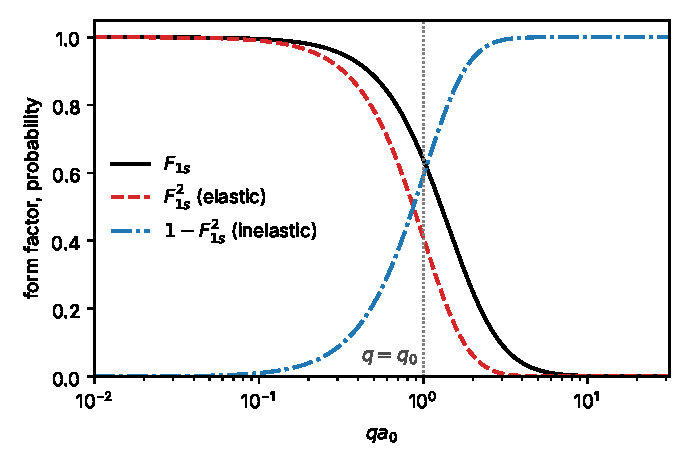
\includegraphics[width=0.62\linewidth]{figures/ch02/fig2_2.pdf}
  \caption{Hydrogen 1s elastic form factor $F_{1s}(q) = 16/(4 + q^2a_0^2)^2$ (solid), its square, the probability that the electron stays in the ground state after absorbing momentum $q$ (dashed), and the probability $1 - F_{1s}^2$ that it is excited or ionized (dash-dotted), against $qa_0$, with $a_0$ the Bohr radius. The dotted line marks the reference momentum $q_0 = \alpha m_e = \SI{3.73}{keV}$, where $qa_0 = 1$ exactly and $F_{1s} = 0.64$. The inelastic probability follows from the closure relation $\sum_f|\langle f|\ee^{\ii\vect{q}\cdot\vect{r}}|1s\rangle|^2 = 1$.}
  \label{fig:2-hydrogen}
\end{figure}

\Cref{fig:2-hydrogen} shows the crossover. Below $q \approx q_0/3$ the atom absorbs the momentum transfer elastically: the electron and the nucleus move together, and the energy deposit is the recoil of the whole atom. Above $q \approx 3q_0$ almost every scattering excites or ionizes the atom. The elastic form factor also explains how a neutral atom hides its charge. A dark photon couples to the electron and to the proton with opposite signs (\cref{sec:1.4}), and the elastic amplitude off the atom is proportional to $1 - F_{1s}(q)$: the proton, a point, contributes $1$, and the electron cloud $-F_{1s}$. At $q \ll q_0$ the two cancel and the dark matter sees a neutral atom; at $q_0$ the squared factor is $(1 - 0.64)^2 = 0.13$. This is screening in its simplest form, and \cref{sec:4.4} treats it in solids.

For ionization the final state is an unbound electron of momentum $p_{\mathrm{ej}}$ and kinetic energy $E_{\mathrm{ej}} = p_{\mathrm{ej}}^2/2m_e$, and the energy transfer is $\omega = E_B + E_{\mathrm{ej}}$, with $E_B > 0$ the binding energy of the shell. Far from the atom the ejected electron is a spherical wave; near it, the wave is distorted by the ion. The sum over final states in \cref{eq:2.2-spectrum} becomes an integral over $p_{\mathrm{ej}}$ and a sum over the angular quantum numbers of the outgoing wave, and the result is conventionally packaged as the \emph{atomic ionization form factor} $|f_{\mathrm{ion}}(p_{\mathrm{ej}}, q)|^2$ of each shell~\cite[Eq.~(6)]{essig2012direct}.

The outgoing waves are labeled by $p_{\mathrm{ej}}$ and by the angular quantum numbers $l', m'$, and normalized to $\langle\tilde\psi_{p'l'm'}|\tilde\psi_{plm}\rangle = (2\pi)^3\delta_{l'l}\delta_{m'm}\,\delta(p' - p)/p^2$. The sum over final states is then $\sum_f = \sum_{l'm'}\int p_{\mathrm{ej}}^2\,\dd p_{\mathrm{ej}}/(2\pi)^3$. With $\dd E_{\mathrm{ej}} = p_{\mathrm{ej}}\,\dd p_{\mathrm{ej}}/m_e$, $p_{\mathrm{ej}}^2\,\dd p_{\mathrm{ej}} = (p_{\mathrm{ej}}^3/2)\,\dd\ln E_{\mathrm{ej}}$. Define
\begin{equation}
  |f_{\mathrm{ion}}(p_{\mathrm{ej}}, q)|^2 = \frac{2p_{\mathrm{ej}}^3}{(2\pi)^3}\sum_{l'm'}\sum_i\left|\int\dd^3r\,\tilde\psi^*_{p_{\mathrm{ej}}l'm'}(\vect{r})\,\psi_i(\vect{r})\,\ee^{\ii\vect{q}\cdot\vect{r}}\right|^2 ,
  \label{eq:2.2-fion}
\end{equation}
with $i$ running over the occupied states of the shell, both spins included. At fixed $E_B$, $\dd\omega = \dd E_{\mathrm{ej}} = E_{\mathrm{ej}}\,\dd\ln E_{\mathrm{ej}}$. In \cref{eq:2.2-spectrum} the delta function $\delta(\omega - E_B - E_{\mathrm{ej}})$ then turns $(p_{\mathrm{ej}}^3/2)\,\dd\ln E_{\mathrm{ej}}$ into $p_{\mathrm{ej}}^3/(2E_{\mathrm{ej}})$, and passing from $\dd/\dd\omega$ to $\dd/\dd\ln E_{\mathrm{ej}}$ multiplies by $E_{\mathrm{ej}}$ again. The sum over final states is therefore $|f_{\mathrm{ion}}|^2/4$ per unit $\ln E_{\mathrm{ej}}$. Inserting this and $|\tilde V|^2 = \pi\sigmae\FDM^2/\mu_{\chi e}^2$ into \cref{eq:2.2-spectrum} leaves the prefactor $(1/2\pi)(\pi\sigmae/\mu_{\chi e}^2)(1/4) = \sigmae/(8\mu_{\chi e}^2)$:
\begin{equation}
  \frac{\dd\langle\sigma v\rangle}{\dd\ln E_{\mathrm{ej}}} = \frac{\sigmae}{8\mu_{\chi e}^2}\int q\,\dd q\,|f_{\mathrm{ion}}(p_{\mathrm{ej}}, q)|^2\,\FDM(q)^2\,\eta(\vmin) , \qquad \vmin = \frac{E_B + E_{\mathrm{ej}}}{q} + \frac{q}{2m_\chi} ,
  \label{eq:2.2-ion}
\end{equation}
the ionization rate of Ref.~\cite[Eqs.~(5) and (6)]{essig2012direct}. It rests on the first Born approximation in the dark-matter potential and treats one electron at a time in a fixed atomic potential, with no correlation and no recoil of the ion.

The exact outgoing waves are tedious to compute, and the standard shortcut replaces them by plane waves. This also shows where the spin factor sits. Replace the outgoing wave by $\ee^{\ii\vect{p}_{\mathrm{ej}}\cdot\vect{r}}$. The overlap in \cref{eq:2.2-ff} is then the momentum-space wavefunction $\tilde\psi_i(\vect{p}_{\mathrm{ej}} - \vect{q})$, with $\tilde\psi_i(\vect{k}) = \int\dd^3r\,\ee^{-\ii\vect{k}\cdot\vect{r}}\psi_i(\vect{r})$. For a full shell, $\sum_m|\tilde\psi_{nlm}(\vect{k})|^2 = (2l + 1)|\tilde\psi_{nl}(k)|^2/4\pi$, where $\tilde\psi_{nl}(k)$ is the radial momentum wavefunction of the shell with principal and orbital quantum numbers $n$, $l$ (Ref.~\cite{essig2012direct} writes $\chi_{nl}$), normalized to $\int k^2\,\dd k\,|\tilde\psi_{nl}|^2 = (2\pi)^3$, and the two spin states double this. The sum over final states is $\int\dd^3p_{\mathrm{ej}}/(2\pi)^3$. At fixed $p_{\mathrm{ej}}$ the integral over its direction relative to $\vect{q}$ becomes an integral over $k = |\vect{p}_{\mathrm{ej}} - \vect{q}|$, since $k^2 = p_{\mathrm{ej}}^2 + q^2 - 2p_{\mathrm{ej}}q\cos\theta'$ gives $2\pi\,\dd\cos\theta' = 2\pi k\,\dd k/(p_{\mathrm{ej}}q)$, with $\theta'$ the angle between $\vect{p}_{\mathrm{ej}}$ and $\vect{q}$ and $k$ running between $|p_{\mathrm{ej}} - q|$ and $p_{\mathrm{ej}} + q$. Collecting the factors as for \cref{eq:2.2-fion},
\begin{equation}
  |f_{\mathrm{ion}}(p_{\mathrm{ej}}, q)|^2_{\mathrm{PW}} = \frac{(2l + 1)\,p_{\mathrm{ej}}^2}{4\pi^3q}\int_{|p_{\mathrm{ej}} - q|}^{p_{\mathrm{ej}} + q}k\,\dd k\,|\tilde\psi_{nl}(k)|^2 ,
  \label{eq:2.2-fion-pw}
\end{equation}
which is the expression given in Ref.~\cite[text after Eq.~(6)]{essig2012direct}; it counts all $2(2l + 1)$ electrons of a full shell, and for the single electron of hydrogen 1s the rate is half of it. The result has a direct reading: the ejected electron leaves with the momentum it had in the atom plus the momentum transfer, and the form factor counts how much of the bound momentum distribution lies on the shell $|\vect{k} + \vect{q}| = p_{\mathrm{ej}}$.

The plane wave ignores the ion. The ion attracts a slow electron and raises its wavefunction near the nucleus, where the overlap with $\psi_i$ is taken, and the effect grows as $E_{\mathrm{ej}}$ falls. For an electron of momentum $p$ leaving a point charge $Z_{\mathrm{eff}}e$, the ratio of the exact to the free probability density at the origin is the Fermi factor familiar from beta decay,
\begin{equation}
  F_{\mathrm{Fermi}}(p) = \frac{2\pi\xi_{\mathrm{C}}}{1 - \ee^{-2\pi\xi_{\mathrm{C}}}} , \qquad \xi_{\mathrm{C}} = \frac{Z_{\mathrm{eff}}\,\alpha m_e}{p} ,
  \label{eq:2.2-fermi}
\end{equation}
which grows as $1/p$ for a slow electron~\cite[Eq.~(1)]{essig2012direct}. Multiplying \cref{eq:2.2-fion-pw} by $F_{\mathrm{Fermi}}(p_{\mathrm{ej}})$ with $Z_{\mathrm{eff}} = 1$ is the standard approximation. For the outer shells of xenon and argon, which dominate their rates, its authors report agreement with continuum states computed in the atomic potential to within $O(\SI{30}{\percent})$ in the total rate~\cite[text after Eq.~(6)]{essig2012direct}. Hydrogen 1s is the one case in which the exact continuum states are known in closed form, and \cref{fig:2-ionization-limit} uses it to test the approximation on a single compact shell. There the same recipe reaches only about half of the exact rate, which does not contradict the xenon and argon result: the quality of the Fermi factor depends on the shell.

\begin{limitbox}[Atomic ionization rate][lim:2.2a]
The ionization rate of a shell with binding energy $E_B$, per unit logarithm of the ejected electron's kinetic energy $E_{\mathrm{ej}} = p_{\mathrm{ej}}^2/2m_e$, is
\begin{gather*}
  \frac{\dd\langle\sigma v\rangle}{\dd\ln E_{\mathrm{ej}}} = \frac{\sigmae}{8\mu_{\chi e}^2}\int q\,\dd q\,|f_{\mathrm{ion}}|^2\,\FDM(q)^2\,\eta(\vmin) ,\\
  |f_{\mathrm{ion}}|^2 \simeq \frac{2\pi\xi_{\mathrm{C}}}{1 - \ee^{-2\pi\xi_{\mathrm{C}}}}\,\frac{(2l + 1)\,p_{\mathrm{ej}}^2}{4\pi^3q}\int_{|p_{\mathrm{ej}} - q|}^{p_{\mathrm{ej}} + q}k\,\dd k\,|\tilde\psi_{nl}(k)|^2 ,
\end{gather*}
with $\xi_{\mathrm{C}} = \alpha m_e/p_{\mathrm{ej}}$ (the Fermi factor of \cref{eq:2.2-fermi} for $Z_{\mathrm{eff}} = 1$), $q$ the momentum transfer, $\tilde\psi_{nl}(k)$ the radial momentum wavefunction of the shell with principal and orbital quantum numbers $n$, $l$, and $\vmin = (E_B + E_{\mathrm{ej}})/q + q/2m_\chi$~\cite[Eqs.~(1), (5) and (6)]{essig2012direct}.
\par\smallskip
{\centering
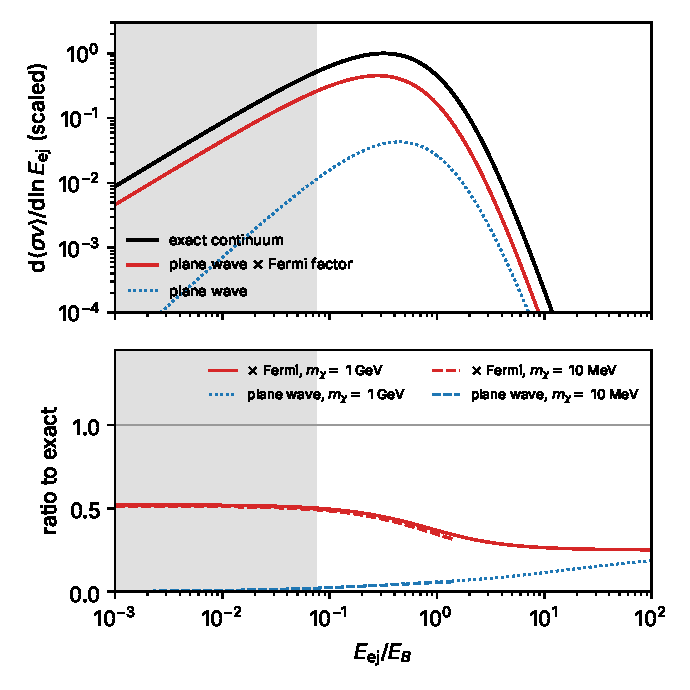
\includegraphics[width=0.8\linewidth]{figures/ch02/limit2_ionization.pdf}
\captionof{figure}{Ionization spectrum of hydrogen 1s (one electron, so half of the two-spin formula above; $E_B = \SI{13.6}{eV}$) for a heavy mediator, $\FDM = 1$, in the standard halo model with the parameters of \cref{tab:1-shm}, against $E_{\mathrm{ej}}/E_B$. Top, for $m_\chi = \SI{1}{GeV}$, scaled to the peak of the exact result: exact Coulomb continuum states (black), plane wave times the Fermi factor with $Z_{\mathrm{eff}} = 1$ (red), plane wave alone (blue dotted). Bottom: the two approximations divided by the exact spectrum, for $m_\chi = \SI{1}{GeV}$ and \SI{10}{MeV}. Gray: $E_{\mathrm{ej}} \le 0.075\,E_B$, where the Fermi-corrected plane wave reaches about half of the exact spectrum. Integrated over $E_{\mathrm{ej}}$ at \SI{1}{GeV}, it gives 0.46 of the exact rate and the plane wave alone 0.036. The exact form factor sums the overlaps with Coulomb partial waves of the hydrogen continuum.}\label{fig:2-ionization-limit}
\par}
\smallskip
Above the shaded region, where most of the rate lies, the halo forces momentum transfers $q \ge (E_B + E_{\mathrm{ej}})/v$ well above $p_{\mathrm{ej}}$, which probe the Coulomb wave at $r \sim 1/q$, where it is not a rescaled plane wave, and the approximation falls to between a quarter and a third of the exact spectrum for $E_{\mathrm{ej}}$ of several $E_B$.
\end{limitbox}

Hydrogen is the only atom with closed-form orbitals. For every other atom the initial orbitals $\psi_i$ are not known exactly: they are computed self-consistently, each electron moving in the average field of the others, as Hartree--Fock orbitals, and the ionization form factors are integrals over them. Ref.~\cite{essig2012direct} used tabulated Roothaan--Hartree--Fock wavefunctions, Hartree--Fock orbitals expanded in a finite set of analytic radial functions; \cref{app:E.7} describes how such form factors are computed and converged, and \cref{sec:3.4} makes the self-consistent-field method precise. In a crystal the same overlap is taken between Bloch states of the valence and conduction bands, summed over their crystal momenta, and the atomic $|f_{\mathrm{ion}}|^2$ becomes the crystal form factor~\cite[Eqs.~(3.13) and (3.17)]{essig2016direct} of \cref{chap:10}.

\subsection{Free electrons}

\Cref{eq:2.2-bound} contains free scattering as a special case, and the check, now in the laboratory frame, shows how the mediator mass enters the free cross-section.

\begin{workedexample}{Scattering off a free electron}\label{we:2-free}
Take an electron at rest, $|i\rangle = |\vect{0}\rangle$, with final states $|f\rangle = |\vect{k}\rangle$ in the box. By \cref{eq:2.2-ff}, $f_{i\to f}(\vect{q}) = \langle\vect{k}|\ee^{\ii\vect{q}\cdot\vect{r}}|\vect{0}\rangle = \delta_{\vect{k}\vect{q}}$: the electron takes exactly the momentum it is given. The sum over $f$ in \cref{eq:2.2-bound} keeps $\vect{k} = \vect{q}$, with $E_f - E_i = q^2/2m_e$, and with $\omega_{\vect{q}} = qv\cos\theta - q^2/2m_\chi$ the delta function is $\delta(q^2/2\mu_{\chi e} - qv\cos\theta)$, where $\theta$ is the angle between $\vect{q}$ and $\vect{v}$ and $1/\mu_{\chi e} = 1/m_e + 1/m_\chi$. Its root is $\cos\theta = q/(2\mu_{\chi e}v)$, which lies in $[-1, 1]$ for $q \le 2\mu_{\chi e}v$, and its weight is $1/(qv)$. With $\dd^3q = 2\pi q^2\,\dd q\,\dd\cos\theta$,
\begin{equation*}
  \sigma_T v = \int_0^{2\mu_{\chi e}v}\frac{2\pi q^2\,\dd q}{(2\pi)^3}\,|\tilde V(q)|^2\,\frac{2\pi}{qv}
  = \frac{1}{2\pi v}\int_0^{2\mu_{\chi e}v}q\,\dd q\,|\tilde V(q)|^2 .
\end{equation*}
Dividing by $v$ gives $\dd\sigma_T/\dd q = q|\tilde V(q)|^2/(2\pi v^2)$, which is \cref{eq:2.2-dsdq}, obtained before in the center-of-mass frame.

For a mediator of mass $m_V$, \cref{eq:1.4-yukawa-sigma} has $\FDM^2 = (m_V^2 + q_0^2)^2/(m_V^2 + q^2)^2$, and the integral over $q^2$ from $0$ to $q_{\mathrm{max}}^2 = (2\mu_{\chi e}v)^2$ is elementary, $\int_0^{q_{\mathrm{max}}^2}\dd x\,(m_V^2 + x)^{-2} = q_{\mathrm{max}}^2/[m_V^2(m_V^2 + q_{\mathrm{max}}^2)]$. So
\begin{equation*}
  \sigma_T = \sigmae\,\frac{(m_V^2 + q_0^2)^2}{m_V^2\,(m_V^2 + q_{\mathrm{max}}^2)} .
\end{equation*}
For concreteness take $m_\chi = \SI{100}{MeV}$, with $\mu_{\chi e} = \SI{0.508}{MeV}$, and the largest halo speed, $v_{\mathrm{max}} = 2.65\times10^{-3}$ (\cref{eq:1.2-vmax}). Then $q_{\mathrm{max}} = \SI{2.69}{keV} = 0.72\,q_0$. A free electron at rest cannot even absorb the reference momentum $q_0$ from such a particle: $\sigmae$ is defined at a momentum transfer that free kinematics does not reach. For a heavy mediator this does not matter. With $m_V = 10\,q_0$ we find $\sigma_T = 1.015\,\sigmae$, and at $m_V = \SI{30}{MeV}$ the difference is $2.3\times10^{-8}$. At $m_V = q_0$, $\sigma_T = 2.63\,\sigmae$, and at $m_V = 0.1\,q_0$, $\sigma_T = 192\,\sigmae$. As $m_V \to 0$ it grows as $q_0^4/(m_V^2q_{\mathrm{max}}^2)$: the free cross-section of a light mediator diverges at small $q$, like Rutherford's, and $\sigmae$ is then just a normalization (\cref{sec:1.4}).
\end{workedexample}

\noindent The free electron at rest is a poor model of a bound one. A bound electron moves with a typical speed $\sim\alpha$, about ten times the dark-matter speed (\cref{sec:1.3}), so it can absorb momentum transfers well above $2\mu_{\chi e}v$, and it needs an energy $E_f - E_i$ that free kinematics does not supply. Both effects sit in $f_{i\to f}$.

For a light mediator the bound target also removes the divergence of \cref{we:2-free}. In \cref{eq:2.2-spectrum} the factor $\FDM^2 = (q_0/q)^4$ multiplies $q\,\dd q$, and the integrand grows as $q^{-3}$ toward small $q$. It stops at $q = \omega/v_{\mathrm{max}}$, below which no dark-matter particle can deposit $\omega$. In addition, the squared form factor of every inelastic transition vanishes at small $q$, as $q^2$ for a dipole-allowed one (\cref{we:2-hydrogen}). The rate is then dominated by the smallest $q$ that kinematics allows, just above the threshold.

\subsection{Nuclei and the Helm form factor}

A nucleus of mass number $A$ is a bound target of $A$ nucleons, and \cref{eq:2.2-ff} applies with one change: every nucleon couples. With a potential $V_N(\vect{x}_\chi - \vect{r}_j)$ between the dark matter and nucleon $j$, the same for protons and neutrons, the target operator is $\sum_{j=1}^A\ee^{\ii\vect{q}\cdot\vect{r}_j}$. Write $\vect{r}_j = \vect{R}_{\mathrm{cm}} + \vect{r}'_j$, with $\vect{R}_{\mathrm{cm}}$ the center of mass of the nucleus and $\vect{r}'_j$ the internal coordinates. The center of mass is a free particle and its plane waves give momentum conservation, as in \cref{eq:2.1-Vbox}. The internal state is the nuclear ground state $|0\rangle$, before and after. The lowest excited levels lie at \SI{1.78}{MeV} in $^{28}$Si, \SI{1.27}{MeV} in $^{29}$Si and \SI{2.24}{MeV} in $^{30}$Si, and between \SI{0.56}{MeV} and \SI{1.04}{MeV} in the even germanium isotopes. The exception is $^{73}$Ge, \SI{7.8}{\percent} of natural germanium, whose first excited state is at \SI{13.3}{keV} and its second at \SI{66.7}{keV}~\cite{iaea2026livechart}. Sub-GeV dark matter carries at most a few keV of kinetic energy (\cref{sec:1.3}), below all of these. The internal matrix element is
\begin{equation}
  \Bigl\langle 0\Bigl|\sum_{j=1}^A\ee^{\ii\vect{q}\cdot\vect{r}'_j}\Bigr|0\Bigr\rangle = \int\dd^3r\;\ee^{\ii\vect{q}\cdot\vect{r}}\,\nd_N(\vect{r}) \equiv A\,F_N(q) ,
  \label{eq:2.2-FN}
\end{equation}
with $\nd_N(\vect{r})$ the nucleon number density of the nucleus, normalized to $\int\dd^3r\,\nd_N = A$, and $F_N(q)$ the \emph{nuclear form factor}, the elastic form factor of the nucleus with $F_N(0) = 1$. This is the coherent sum: at $q \to 0$ the phases of all nucleons agree and the amplitude is $A$ times that of one nucleon. The two-body result \cref{eq:2.2-dsdq}, with $\mu_{\chi e} \to \mu_{\chi N}$ and $\tilde V \to A\tilde V_N F_N$, gives
\begin{equation}
  \frac{\dd\sigma_N}{\dd q} = \frac{q\,A^2|\tilde V_N(q)|^2}{2\pi v^2}\,F_N(q)^2
  = \frac{q\,\sigma_N}{2\mu_{\chi N}^2v^2}\,F_N(q)^2 , \qquad
  \sigma_N = \frac{\mu_{\chi N}^2A^2|\tilde V_N|^2}{\pi} = \sigma_p\left(\frac{\mu_{\chi N}}{\mu_{\chi p}}\right)^2A^2 ,
  \label{eq:2.2-nucleus}
\end{equation}
for a heavy mediator, $\tilde V_N = y_\chi y_N/m_V^2$. The expression through $\sigma_p$ uses the proton cross-section $\sigma_p = \mu_{\chi p}^2|\tilde V_N|^2/\pi$, which is \cref{eq:2.2-sigma-free} with $\mu_{\chi e} \to \mu_{\chi p}$. This derives \cref{eq:1.4-sigmaN}, and $\sigma_N$ is the cross-section at $q \to 0$; the form factor then cuts off the distribution at large $q$. Unequal proton and neutron couplings replace $A$ by $Z + (A - Z)y_n/y_p$ (\cref{sec:1.4}).

Experiments measure the recoil energy $E_R = q^2/2M$ rather than $q$, with $M$ the nuclear mass. With $\dd E_R = q\,\dd q/M$, $\dd\sigma_N/\dd E_R = M\sigma_NF_N^2/(2\mu_{\chi N}^2v^2)$. We multiply by the number of nuclei per unit mass, $1/M$, and by the dark-matter flux $(\rho_\chi/m_\chi)\,v\,f_\chi(\vect{v})\,\dd^3v$. Integrating over velocities above $\vmin = (ME_R/2\mu_{\chi N}^2)^{1/2}$ (\cref{sec:1.3}) then turns the factor $v/v^2$ into $\eta(\vmin)$:
\begin{equation*}
  \frac{\dd\mathcal{R}}{\dd E_R} = \frac{\rho_\chi\,\sigma_N}{2m_\chi\mu_{\chi N}^2}\,F_N(q)^2\,\eta(\vmin) , \qquad q = (2ME_R)^{1/2} ,
\end{equation*}
the standard spin-independent recoil spectrum, Ref.~\cite[Eq.~(104)]{lin2019tasi} with $\sigma_N$ written through \cref{eq:1.4-sigmaN} and equal couplings to protons and neutrons.

The nucleon density is close to uniform inside the nucleus and falls off over a skin about \SI{1}{fm} thick. Helm's model~\cite{helm1956inelastic} writes it as a uniform sphere of radius $R_{\mathrm{nuc}}$ smeared by a Gaussian of width $s_{\mathrm{skin}}$. The transform of a convolution is the product of the transforms. For the uniform sphere, the angular integral is $4\pi\sin(qr)/(qr)$ again (\cref{app:C.3}), and $\int_0^{R}\dd r\,r\sin qr = (\sin qR - qR\cos qR)/q^2$, so its normalized transform is $3(\sin x - x\cos x)/x^3 = 3j_1(x)/x$ with $x = qR_{\mathrm{nuc}}$ and $j_1$ the spherical Bessel function. The normalized Gaussian $\ee^{-r^2/2s_{\mathrm{skin}}^2}/(2\pi s_{\mathrm{skin}}^2)^{3/2}$ transforms to $\ee^{-q^2s_{\mathrm{skin}}^2/2}$. Multiplying the two gives~\cite[Eq.~(17)]{duda2007model}
\begin{equation}
  F_{\mathrm{Helm}}(q) = \frac{3j_1(qR_{\mathrm{nuc}})}{qR_{\mathrm{nuc}}}\,\ee^{-q^2s_{\mathrm{skin}}^2/2} .
  \label{eq:2.2-helm}
\end{equation}
The standard parameters are those of Lewin and Smith~\cite{lewin1996review}: $R_{\mathrm{nuc}}^2 = c_{\mathrm{nuc}}^2 + \tfrac73\pi^2a_{\mathrm{nuc}}^2 - 5s_{\mathrm{skin}}^2$, with $c_{\mathrm{nuc}} = (1.23A^{1/3} - 0.60)\,\si{fm}$, $a_{\mathrm{nuc}} = \SI{0.52}{fm}$ and $s_{\mathrm{skin}} = \SI{0.9}{fm}$~\cite[Eqs.~(11) and (12), quoting Lewin and Smith]{duda2007model}. Here $c_{\mathrm{nuc}}$ and $a_{\mathrm{nuc}}$ are the half-density radius and surface diffuseness of a Woods--Saxon density, and the formula for $R_{\mathrm{nuc}}$ matches the Helm form to it. The literature writes $r_n$ or $R_1$ for $R_{\mathrm{nuc}}$, $s$ for $s_{\mathrm{skin}}$, and $c$, $a$ for $c_{\mathrm{nuc}}$, $a_{\mathrm{nuc}}$. At small $q$, $3j_1(x)/x \simeq 1 - x^2/10$ and $F_{\mathrm{Helm}} \simeq 1 - q^2(R_{\mathrm{nuc}}^2/10 + s_{\mathrm{skin}}^2/2)$, the form $1 - q^2\langle r^2\rangle/6$ with $\langle r^2\rangle = \tfrac35R_{\mathrm{nuc}}^2 + 3s_{\mathrm{skin}}^2$. For silicon, $c_{\mathrm{nuc}} = \SI{3.14}{fm}$ and $R_{\mathrm{nuc}} = \SI{3.47}{fm}$; for germanium ($A = 73$), $c_{\mathrm{nuc}} = \SI{4.54}{fm}$ and $R_{\mathrm{nuc}} = \SI{4.77}{fm}$. The simpler fit $R_{\mathrm{nuc}} \approx 1.14A^{1/3}$\,fm of Ref.~\cite[Sect.~IV\,C]{lin2019tasi} yields \SI{3.46}{fm} and \SI{4.76}{fm}, the same to within a percent.

The Helm form is a model, not a measurement. Electron scattering measures the charge density of the nucleus, that is, the protons. The form factor of \cref{eq:2.2-FN} needs the density of all nucleons. The standard assumption is that the two are proportional, in which case the nucleon form factor equals the charge form factor~\cite[Eqs.~(7) and (8)]{duda2007model}; for the dark photon, which couples to charge, the charge form factor is exact. The physical form factor is then the transform of the measured charge density, and Ref.~\cite[Sect.~V]{duda2007model} compares the two. For $^{28}$Si the Lewin--Smith Helm form factor differs from the measured one negligibly at small $q$ and by up to \SI{5}{\percent} at the momentum transfer of a \SI{100}{keV} recoil; for $^{70}$Ge the difference is \SI{2}{\percent} at \SI{10}{keV} and \SI{20}{\percent} at \SI{100}{keV}. We use the Helm form as the convention of the field, and it is accurate wherever light dark matter is concerned.

\begin{figure}[tbp]
  \centering
  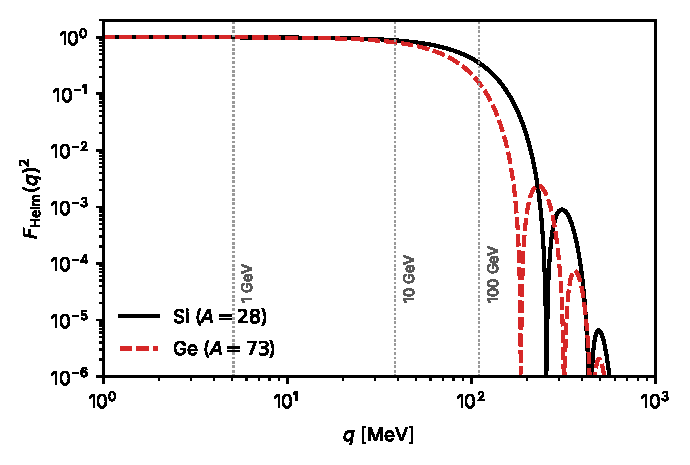
\includegraphics[width=0.62\linewidth]{figures/ch02/fig2_3.pdf}
  \caption{Squared Helm nuclear form factor $F_{\mathrm{Helm}}(q)^2 = [3j_1(qR_{\mathrm{nuc}})/(qR_{\mathrm{nuc}})]^2\ee^{-q^2s_{\mathrm{skin}}^2}$ of silicon ($A = 28$, solid) and germanium ($A = 73$, the integer nearest the mean mass number 72.6 of natural germanium; dashed), against the momentum transfer $q$. Parameters of Lewin and Smith: $R_{\mathrm{nuc}}^2 = c_{\mathrm{nuc}}^2 + \tfrac73\pi^2a_{\mathrm{nuc}}^2 - 5s_{\mathrm{skin}}^2$, $c_{\mathrm{nuc}} = (1.23A^{1/3} - 0.60)\,\si{fm}$, $a_{\mathrm{nuc}} = \SI{0.52}{fm}$, $s_{\mathrm{skin}} = \SI{0.9}{fm}$, which give $R_{\mathrm{nuc}} = \SI{3.47}{fm}$ (Si) and \SI{4.77}{fm} (Ge). Dotted lines: the maximum momentum transfer $2\mu_{\chi N}v_{\mathrm{max}}$ to a silicon nucleus for dark-matter masses of 1, 10 and \SI{100}{GeV}, with $v_{\mathrm{max}} = \SI{794.5}{km/s}$. The first zero is at $qR_{\mathrm{nuc}} = 4.49$, the first zero of $j_1$: $q = \SI{256}{MeV}$ for Si and \SI{186}{MeV} for Ge.}
  \label{fig:2-helm}
\end{figure}

\Cref{fig:2-helm} shows that light dark matter never resolves the nucleus. The silicon radius $R_{\mathrm{nuc}} = \SI{3.47}{fm}$ corresponds to $1/R_{\mathrm{nuc}} = \SI{57}{MeV}$, and germanium's \SI{4.77}{fm} to \SI{41}{MeV}. The form factor matters once $qR_{\mathrm{nuc}}$ approaches one, at tens of MeV, which needs dark matter of several GeV.

\begin{workedexample}{The $A^2$ enhancement for silicon}\label{we:2-coherent}
For $^{28}$Si, $A^2 = 784$. With the mean atomic mass of natural silicon, \SI{26.16}{GeV}, the reduced masses at $m_\chi = \SI{100}{MeV}$ are $\mu_{\chi p} = \SI{90.4}{MeV}$ and $\mu_{\chi N} = \SI{99.6}{MeV}$, and \cref{eq:2.2-nucleus} gives $\sigma_N/\sigma_p = 1.215 \times 784 = 953$; at \SI{1}{GeV}, $\mu_{\chi p} = \SI{484}{MeV}$, $\mu_{\chi N} = \SI{963}{MeV}$, and $\sigma_N/\sigma_p = 3.96 \times 784 = 3100$. Coherence turns the $A$ of 28 nucleons scattering independently into $A^2$, a gain of 28; the reduced-mass factor is a separate effect of the heavier recoiling target. Per kilogram of target the rate still grows as $A$, because $A^2$ in the cross-section beats the $1/A$ in the number of nuclei per unit mass. The form factor costs almost nothing. At $m_\chi = \SI{1}{GeV}$ the maximum momentum transfer is $q_{\mathrm{max}} = 2\mu_{\chi N}v_{\mathrm{max}} = \SI{5.10}{MeV}$ (\cref{we:1-nuclear}), and $q_{\mathrm{max}}R_{\mathrm{nuc}} = 0.090$ and $F_{\mathrm{Helm}}^2 = 0.998$ at the maximum momentum transfer, where the suppression is greatest. The same calculation yields $F_{\mathrm{Helm}}^2(q_{\mathrm{max}}) = 0.89$ at \SI{10}{GeV} and $0.36$ at \SI{100}{GeV}. For germanium at \SI{100}{GeV}, $q_{\mathrm{max}} = \SI{214}{MeV}$ lies beyond the first zero and $F_{\mathrm{Helm}}^2 = 0.002$ there. Form factors shape the recoil spectra of weak-scale dark matter but are a \SI{0.2}{\percent} correction at \SI{1}{GeV} and far less for the sub-GeV dark matter of this book.
\end{workedexample}
